\chapter{Protocolli epidemici nel dettaglio}
Un protocollo epidemico è un modello di comunicazione che trae ispirazione dallo studio della diffusione di epidemie. In modo intercambiabile si può utilizzare il termine protocollo di gossip, derivante dall'omonimo fenomeno studiato nell'ambito delle scienze sociali come metodo efficace per il passaggio di informazioni in una rete sociale.

Il gossip e le epidemie sono stati analizzati e le loro caratteristiche sono state implementate in reti informatiche, nello specifico in sistemi distribuiti. Le regole su cui si basa il loro funzionamento sono semplici, ma allo stesso tempo sono robusti veloci ed affidabili. Inoltre, non è necessario alcun controllo centralizzato, condizione necessaria affinché possano essere utilizzati nei sistemi distribuiti

\section{Storia}
I protocolli epidemici vengono analizzati per la prima volta in un documento scritto da Alan Demers \cite{demers} nel 1987. Il problema riscontrato da Demers e dai suoi colleghi nella rete interna del centro di ricerca di Xerox a Palo Alto era il seguente: mantenere la consistenza tra più copie di un database presente nelle diverse macchine. Il loro obiettivo consisteva nel progettare algoritmi robusti, efficienti e con elevata scalabilità, tenendo conto del tempo necessario per la distribuzione di un aggiornamento in una rete ed il traffico generato. Dopo aver esaminato un protocollo best-effort chiamato direct mail, che prevede l'invio in broadcast a tutti i nodi di una rete dell'aggiornamento ricevuto ed aver notato che non era efficiente né affidabile (è possibile che un messaggio venga perso e non è sempre scontato che un nodo conosca tutti i componenti in una rete), le loro attenzioni si sono spostate verso due tipologie di protocolli epidemici: anti-entropy e rumor-mongering. Entrambi prevedono lo scambio periodico di informazioni tra nodi scelti in modo casuale, cercando di risolvere le differenze che intercorrono tra i due database dei rispettivi end-point. Attraverso questi approcci si può ottenere consistenza eventuale (eventual consistency), una forma di consistenza debole, tale per cui un sistema di storagee garantisce che se non ci sono ulteriori aggiornamenti, tutti gli accessi ritorneranno il valore più aggiornato \cite{vogels}.

I protocolli di gossip sono utilizzati oggigiorno in numerosi contesti: in sistemi peer-to-peer che necessitano di scambio di informazioni, come il sistema di condivisione di file BitTorrent [bittorrent] oppure nella rete BitCoin [serve fonte se possibile, ho trovato solo forum che ne parlano].

\section{Information dissemination}
La prima applicazione che verrà analizzata riguarda la distribuzione di informazioni, come avviene naturalmente nel gossip. Gossip nei sistemi distribuiti significa scambiarsi informazioni in modo periodico e probabilistico tra due membri \cite{kermarrec}. È importante notare che questo processo viene eseguito ripetutamente e di per se non ha una condizione di terminazione, ma verrà introdotta parlando del modello SIR e degli algoritmi di rumor-mongering.
\subsection{Componenti e notazione}
Si consideri una rete composta da un numero fissato P di nodi. Il grafo generato sarà completo, ovvero ogni nodo potrà comunicare direttamente con tutti gli altri nodi. Ogni nodo contiene una variabile chiamata \textit{value} inizialmente uguale per tutti. I nodi potranno scambiarsi messaggi contenenti \textit{value}, la quale avrà un attributo \textit{value.timestamp} che indicherà la data e l'ora dell'ultimo aggiornamento. L'obiettivo di questi algoritmi sarà: in assenza di ulteriori aggiornamenti, \textit{value} sarà uguale in tutti i nodi.

Ogni nodo possiede anche un attributo status che potrà assumere tre valori, ispirati alla terminologia utilizzata in epidemiologia:
\begin{itemize}
    \item \textbf{Susceptible}(S): un nodo che non è venuto a conoscenza di un aggiornamento
    \item \textbf{Infected}(I): un nodo che è venuto a conoscenza dell'aggiornamento e lo sta distribuendo attivamente
    \item \textbf{Removed}(R): un nodo che è venuto a conoscenza dell'aggiornamento ma non lo distribuisce più
\end{itemize}
Gli stati \textit{susceptible} e \textit{infected} verranno utilizzati nel modello SI, mentre aggiungendo lo stato \textit{removed} si parlerà di modello SIR.
\subsection{Epidemie semplici}

\begin{figure}[!htb]
    \begin{subfigure}{0.32\textwidth}
      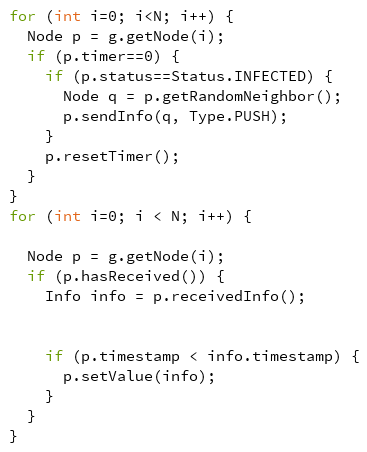
\includegraphics[width=\linewidth,height=8cm]{push-code.png}
      \caption{Push}\label{fig:push_code}
    \end{subfigure}\hfill
    \begin{subfigure}{0.32\textwidth}
      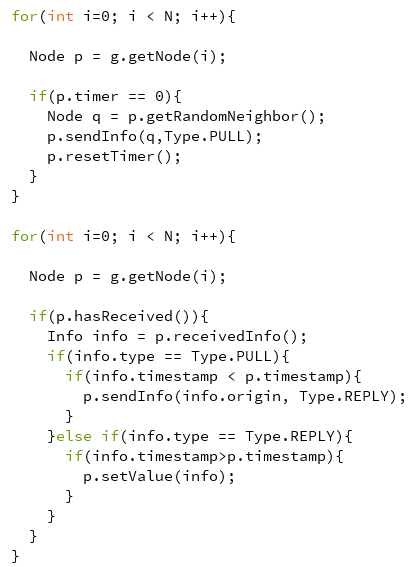
\includegraphics[width=\linewidth, height=8cm]{pull-code.png}
      \caption{Pull}\label{fig:pull_code}
    \end{subfigure}\hfill
    \begin{subfigure}{0.32\textwidth}
      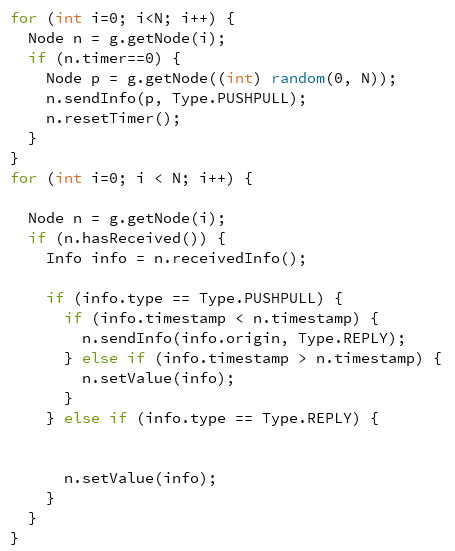
\includegraphics[width=\linewidth, height=8cm]{pushpull-code.png}
      \caption{Pushpull}\label{fig:pushpull_code}
    \end{subfigure}
    \caption{Epidemie semplici}
    \label{fig:simple_epidemics}
    \end{figure}
Il modello SI, chiamato anche anti-entropy o delle epidemie semplici, è il primo protocollo studiato nel centro di ricerca di Xerox. Come già detto, un nodo potrà trovarsi nello stato \textit{susceptible} o \textit{infected}. L'invio periodico di informazioni è scandito da un timer proprio del nodo, impostato inizialmente al valore $\Delta$. Quando il timer scende a zero, il nodo invia il messaggio secondo lo stile scelto ed imposta nuovamente il timer. È interessante notare ogni nodo esegue queste operazioni una sola volta per round.

Nel documento originale vengono esposti e studiati tre stili per il modello SI, che cambiano il modo in cui i componenti della rete comunicano e risolvono le differenze. 

Si utilizzerà la seguente notazione: $n$ indica il numero totale dei nodi presenti sulla rete ($|P|$), mentre i valori $s$ e $i$ indicano rispettivamente il rapporto $|S|/n$ e $|I|/n$. Chiaramente $s + i = 1$.
\subsubsection{Push}
Il primo stile è detto stile push: un nodo infetto sceglierà in modo casuale un vicino a cui inviare informazioni. il nodo destinazione verificherà se le informazioni ricevute sono più aggiornate e, in caso affermativo, cambierà il proprio valore. Un nodo quindi, se infetto, invierà sempre un messaggio ad un altro nodo, indipendentemente dal fatto che il nodo destinazione conosca o meno l'aggiornamento. Si può facilmente intuire che lo stile push è più efficace quando il numero di nodi infetti è basso. In uqesta situazione, infatti, il numero di nodi infetti tenderà a raddoppiare ad ogni round e dopo $O(\log_2 n)$ round il valore $i$ si avvicinerà a $1/2$. Quando invece $i$ supera $1/2$ la situazione cambia: se definiamo $s_t$ il rapporto di nodi suscettibili al roud $t$, possiamo calcolare il numero atteso di nodi suscettibili al round $t + 1$ come:
\begin{equation}
    E(s_{t + 1}) = s_t  \Big(1 - \frac{1}{n}\Big)^{n(1-s_t)}
\end{equation}
Nel dettaglio: un nodo rimane suscettibile se al round $t$ era suscettibile ($s_t$) e non è stato contattato da nessuno dei nodi infetti ($1-1/n$ indica la probabilità che un nodo non contatti il nodo suscettibile, ripetuto per il numero di nodi infetti $n(1-s_t)$).

Questo valore può essere approssimato per $n$ molto grandi a $s_t e^{-(1-s_t)}$. Come dimostra Pittel \cite{pittel} il numero di round atteso $T(n)$ per informare tutti i nodi in una rete è
\begin{equation}
    T(n)= \log_2 n + \ln n + O(1) = O(\log n)
\end{equation}

dove $\log_2 n$ deriva dalla prima fase, $\ln n$ da quella finale, mentre la fase intermedia, molto veloce, dura un numero costante di cicli.
\subsubsection{Pull}
Il secondo stile analizzato è lo stile pull: i nodi chiedono informazioni ad altri nodi, inviando il proprio timestamp. Se questi ultimi possiedono un aggiornamento più recente, invieranno un messaggio in risposta che verrà utilizzato dal nodo iniziale per cambiare il proprio valore.

A differenza dello stile push, quest'ultimo risulta poco efficace quando i nodi infetti sono pochi. Il numero atteso di nodi non ancora infeti dopo $t+1$ round può essere espresso come:
\begin{equation}
    E(s_{t+1}) = s_t \cdot s_t = s_t^2
\end{equation}
in quanto un nodo rimane non informato se nel round precedente era suscettibile ed ha contattato un nodo a sua volta suscettibile. Può accadere che un nodo infetto dovrà aspettare alcuni round prima di venir contattato, rendendo questi round inutili per lo scopo dell'algoritmo. Nonostante ciò, con alta probabilità dopo $O(log n)$ round metà dei nodi sarà infetta. La fase finale invece è molto più rapida in quanto, aumentando il numero di nodi infetti, aumenta la probabilità per un nodo suscettibile di contattare un nodo infetto.
\subsubsection{Push-Pull}
La soluzione migliore proposta si basa su una combinazione dei due stili precedenti. Lo stile push-pull lavora nel modo seguente: all’azzeramento del timer, un nodo invia un messaggio ad un altro nodo scelto tra i vicini in modo casuale, il quale controllerà il timestamp ed a seconda del risultato invierà una risposta oppure aggiornerà il proprio valore. E’ più rapido in quanto sfrutta i punti di forza dei protocolli push e pull (nella fase iniziale sfrutterà il push, nella parte finale il pull). Karp \cite{karp} ha dimostrato che il numero atteso di round per infettare tutti i nodi è $O(\log\log n)$.

Riassumendo, il modello SI è efficace in quanto permette di distribuire su tutta la rete un aggiornamento, in quanto un nodo infetto continuerà (idealmente per sempre) ad inviare o ricevere messaggi. Nonostante ciò questo può rivelarsi un peso non indifferente per la rete in quanto questo modello prevede l’invio del database completo all’interno del messaggio e non il singolo aggiornamento. Se gli aggiornamenti in una rete sono rari, la maggior parte dei messaggi diventa inutile, perché i nodi continueranno a contattarne altri che già sono a conoscenza  dell’aggiornamento. 
\subsection{Epidemie complesse}

\begin{figure}[!htb]
    \begin{subfigure}{0.40\textwidth}
      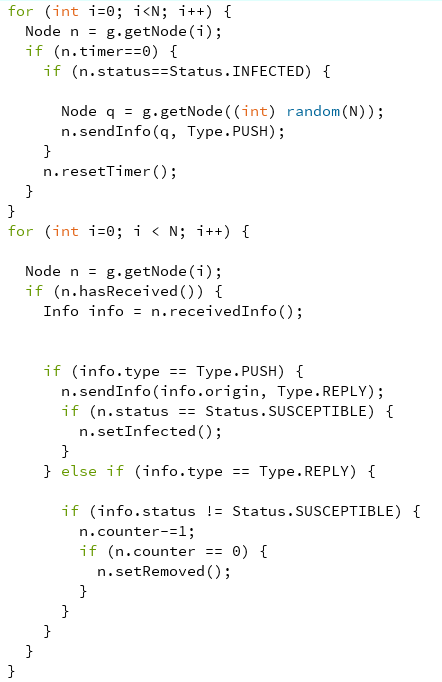
\includegraphics[width=\linewidth,height=10cm]{feedback-counter-code.png}
      \caption{Feedback Counter}\label{fig:feedback_counter_code}
    \end{subfigure}\hfill
    \begin{subfigure}{0.40\textwidth}
      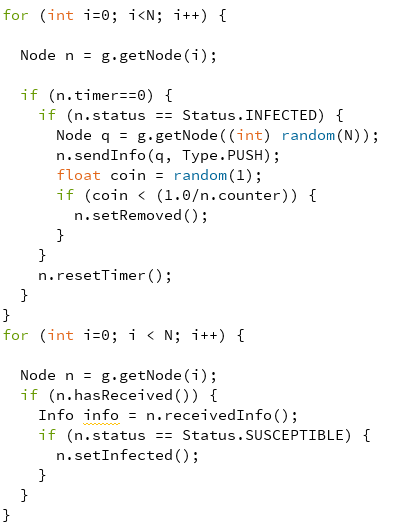
\includegraphics[width=\linewidth, height=10cm]{blind-coin-code.png}
      \caption{Blind Coin}\label{fig:blind_coin_code}
    \end{subfigure}\hfill
    \caption{Epidemie complesse}
    \label{fig:simple_epidemics}
    \end{figure}
Il modello SIR viene introdotto per risolvere il problema della non terminazione del modello precedente e per aumentare l’efficienza. I nodi potranno assumere lo stato rimosso, ovvero nodi che conoscono l’aggiornamento ma non lo distribuiscono più.
Come per le epidemie semplici, inizialmente i nodi sono tutti suscettibili: quando uno di questi viene a conoscenza di un aggiornamento, diventa infetto ed incomincia ad inviare messaggi agli altri nodi. Eventualmente questi nodi potranno “perdere” interesse nel distribuire il proprio aggiornamento, cambiando così il suo stato in rimosso.
Quando nella rete non ci sarà più nessun nodo infetto, l’algoritmo termina.
Il passaggio dallo stato infetto allo stato rimosso può essere influenzato dai seguenti fattori:

\begin{itemize}
    \item \textbf{Come} (How):
    \begin{itemize}
        \item \textbf{counter}: un nodo passerà allo stato rimosso dopo $k$ contatti
        \item \textbf{coin}: un nodo passerà allo stato rimosso con probabilità $1/k$

    \end{itemize}
    \item \textbf{Quando} (When)
    \begin{itemize}
        \item \textbf{feedback}: la valutazione avverrà quando un nodo contatta un altro nodo che era già a conoscenza dell’aggiornamento
        \item \textbf{blind}: la valutazione avverrà ad ogni round
    \end{itemize}
\end{itemize}

Si ottengono così quattro possibili combinazioni: \textit{
feedback/counter, blind/coin, feedback/coin, blind/counter}.
Verranno analizzati \textit{feedback/counter} e \textit{blind/coin} utilizzando lo stile push, ma le considerazioni potranno essere applicate allo stesso modo anche per gli altri algoritmi.

Per confrontare i diversi protocolli che si basano sul modello SIR si utilizzano i seguenti criteri:
\begin{itemize}
    \item \textbf{Residuo}: indica il numero di nodi ancora suscettibili al termine dell’algoritmo (viene indicato con $s^*$). Non è garantito infatti, come invece accade nel modello SI, che tutti i nodi verranno a conoscenza dell’aggiornamento. Può verificarsi una situazione in cui tutti i nodi si trovano nello stato suscettibile oppure rimosso, senza quindi aver ottenuto consistenza in tutta la rete.
    \item \textbf{Traffico}: indica il numero di messaggi inviati. Spesso si utilizza il traffico medio, definito come
    \begin{equation}
        m = \frac{\textrm{traffico totale}}{\textrm{numero di nodi}}        
    \end{equation}
    \item \textbf{Ritardo}: può essere espresso come ritardo medio $t_{avg}$, ovvero la differenza tra il momento dell'infezione iniziale e l'arrivo di un aggiornamento, mediato sul numero di nodi, oppure come ritardo totale $t_{max}$, cioè il tempo necessario affinché l'ultimo nodo riceva l'aggiornamento.
\end{itemize}  
Definiamo, come per il modello SI, $s$, $i$ e $r$ come la il rapporto di nodi suscettibili, infetti e rimossi rispetto al numero di nodi, in modo tale che $s + i + r = 1$.

L’andamento dei seguenti algoritmi può essere modellato attraverso l’utilizzo delle seguenti equazioni differenziali \cite{hethcote}:
\begin{equation}
    \begin{split}
        \frac{ds}{dt} & = - \beta is \\
    \frac{di}{dt} & = \beta is - \gamma i \\
    \frac{dr}{dt} & = \gamma i
    \end{split}
\end{equation}

dove $\beta$ rappresenta il tasso di contagio mentre $\gamma$, chiamato in epidemiologia tasso di recupero, è un valore che dipende da $k$ e dal numero di nodi ancora suscettibili, più precisamente
\begin{equation}
    \gamma = \frac{1}{k}(1-s)
\end{equation}

Possiamo utilizzare le prime due per risolvere il sistema di equazioni differenziali partendo dal loro rapporto e supponendo beta uguale a 1:
\begin{equation}
    \begin{split}
        \frac{di}{ds}   & =  \frac{si - \frac{1}{k} (1-s) i}{-si} \\
        & = \frac{\frac{\cancel{i} (ks - 1 + s)}{k}}{- \cancel{i}s} \\
        & = \frac{1-ks-s}{ks} \\
        & = \frac{1}{ks} - 1 - \frac{1}{k} \\
        & = \frac{1}{ks} - \frac{1+k}{k} 
    \end{split}
\end{equation}
integrando si ottiene
\begin{equation}
    s(i) = \frac{1}{k} \ln s - \frac{1+k}{k} + c
\end{equation}
dove c è costante di integrazione che si può calcolare considerando che inizialmente la funzione è espressa come $i(1-1/n) = 1/n$ che tende a $0$ per $n$ molto grandi

\begin{equation}
    c = \frac{k+1}{k}
\end{equation}
che porta alla seguente soluzione

\begin{equation}
    i(s) = \frac{k+1}{k}(1-s) + \frac{1}{k} \ln s
\end{equation}
Questa equazione può essere utilizzata per calcolare $s^*$ quando $i(s^*) = 0$

\begin{equation}
    s^* = e^{(-k-1)(1-s^*)}
\end{equation}

Il risultato è una funzione implicita su $s^*$, la quale mostra che il residuo diminuisce esponenzialmente all'aumentare di $k$.

È possibile notare inoltre che tutte le varianti dell’algoritmo condividono la stessa relazione tra traffico e residuo. Considerando ogni messaggio inviato ha probabilità pari a 1/n di contattare un nodo specifico, la probabilità di rimanere suscettibile dopo l’invio di m*n messaggi è pari a:

\begin{equation}
    s(m*n) = \Big(1-\frac{1}{n}\Big)^{nm}
\end{equation}

che con $n$ grandi può essere approssimato come $s = e^{-m}$.
Come si può notare dalla tabella 1, il ritardo è l’unico parametro che distingue le varianti: osservando i dati si può notare che feedback/counter offre ritardo inferiore a parità di $k$.




\subsection{Dettagli implementativi}

Nelle pagine precedenti sono stati descritti i protocolli basati sui modelli SI e SIR utilizzati per la distribuzione di informazioni, senza parlare di come questi possano essere utilizzati in casi reali. Innanzitutto anti-entropy e rumor-mongering possono essere utilizzati in contemporanea sulla medesima rete: si suppone infatti che un protocollo basato sul modello SIR può eventualmente terminare senza che si sia ottenuta consistenza su tutta la rete. Per evitare che ciò accada, è possibile eseguire un algoritmo anti-entropy meno frequentemente.


\subsubsection{Valori multipli}

È molto probabile che i protocolli debbano lavorare con più che singoli valori, e quindi la comparazione può diventare molto onerosa. Molto spesso infatti, lavorando con database per esempio, il confronto diventa quasi completamente inutile perché gran parte dei dati sono simili. È possibile risolvere in parte questo problema utilizzando dei checksum calcolati a partire dalla copia del database contenuta nel nodo, ricalcolando ogni volta che quest’ultimo viene aggiornato. Il primo scambio tra nodi avviene attraverso il confronto dei relativi checksum, eseguendo il confronto completo dei database solo se si trovano in disaccordo. Purtroppo la computazione dei checksum tende ad essere molto spesso diversa se l’aggiornamento ai nodi arriva in momenti tanto diversi, quindi la rete tenderà comunque a dover confrontare i dati completi. Una soluzione più complessa prevede di definire un intervallo di tempo che sia sufficiente per far ricevere l’aggiornamento a tutti i nodi. Ogni nodo contiene una lista con gli aggiornamenti più recenti, all’interno di questo spazio di tempo, che viene scambiata ed utilizzata per aggiornare checksum e database. Solo nel caso di un ulteriore disaccordo, viene eseguito il confronto con l’intero database. È importante notare che la scelta dell’intervallo di tempo è cruciale per il funzionamento: se viene fatta in maniera sbagliata, i checksum tenderanno a differenziarsi, aumentando il traffico rendendolo superiore al traffico generato dai protocolli anti-entropy senza checksum.

Un' ultima soluzione, che non prevede la scelta a priori di un intervallo di tempo, prevede la memorizzazione di un indice inverso del database basato sul timestamp. I nodi si scambiano gli aggiornamenti in ordine inverso di timestamp, ricalcolando i checksum fino ad ottenere un consistenza di questi ultimi. Non è comunque ottimale a causa del costo di mantenimento dell’indice inverso in ogni nodo.

\subsubsection{Traffico generato}
Un problema non trascurabile in casi reali è sicuramente il traffico che una rete può supportare. Questi protocolli prevedono che ad ogni round vengano inviati più messaggi contemporaneamente, rischiando quindi di sovraccaricare la rete. Demer aveva definito questo come connection limit, spiegando che definire un limite è necessario sia in caso di puh che di pull. Questa condizione porta però ad un significativo peggioramento dei protocolli che utilizzano lo stile pull, mentre push diventa migliore. Il protocollo Scuttlebutt \cite{flowgossip} definisce alcuni rimedi a questa limitazione, specificando un metodo per determinare in modo dinamico il tasso massimo di traffico che un nodo può generare senza dover creare un sistema di backlog per gli aggiornamenti. 

\subsubsection{Gestione dei fallimenti}
Implementando i protocolli di gossip in contesti reali comporta il rischio di possibili fallimenti per fattori esterni. Per fortuna, la perdita di messaggi non aggrava sull’esecuzione se non rallentando il raggiungimento della consistenza (alcuni round diventano inutili). Se alcuni nodi smettono di “funzionare”, gli scambi con questi diventano inutili e i protocolli rallentano la loro esecuzione. È comunque auspicabile mantenere lo stato attivo degli endpoint in modo da evitare questi inconvenienti.

\section{Altri utilizzi dei protocolli epidemici}

Negli scritti di Demers \cite{demers}, si supponeva che la rete fosse statica, ovvero il numero di nodi rimaneva fisso nel tempo. Inoltre ogni nodo aveva una visione totale, e quindi il grafo rappresentativo era completo. Infine il numero di macchine collegate era relativamente basso.
Oggigiorno le reti sono molto più grandi, non sono completamente connesse e la lista di nodi direttamente connessi tra loro può variare per continue connessioni-disconnessioni. Questo sicuramente porta grandi vantaggi, come una maggior scalabilità. I protocolli epidemici possono essere adattati a questi grandi cambiamenti ed utilizzati per altri scopi, oltre alla distribuzione di informazioni. Esistono implementazioni dei protocolli epidemici per mantenere informazioni sullo stato di una rete peer-to-peer \cite{newscast}, per rilevare errori e guasti \cite{swim}, per implementare garbage collection \cite{garbage_collection}, per calcolare informazioni di aggregazione \cite{aggregation}, …
\subsection{Notazione}

Si può definire un algoritmo di gossip generico, che si basa sulle implementazioni precedenti e descrive i vari momenti che devono essere tenuti in considerazione:
\begin{itemize}
    \item \textbf{inizializzazione}: un nodo viene definito con il suo stato iniziale. Viene impostato il timer
    \item \textbf{allo scadere del timer}: il nodo sceglie un vicino, prepara il messaggio, lo invia al nodo scelto e reimposta il timer
    \item \textbf{al ricevimento di un messaggio di richiesta}: il nodo prepara la risposta e la invia. Il nodo legge la richiesta e la elabora
    \item \textbf{al ricevimento di un messaggio di risposta}: il nodo elabora la risposta.
\end{itemize}

Da queste situazioni si può notare come i metodi di elaborazione ed invio non sono stati implementati, ma questa operazione verrà fatta in seguito. 

\section{Peer sampling}

Per la gestione di reti dinamiche e di grandi dimensioni, il mantenimento di una lista contenente tutti i nodi è oneroso e per nulla efficiente. A causa della possibilità di fallimenti o di nuovi nodi, questa lista deve essere aggiornata frequentemente, per poi essere diffusa a tutti. 

Per risolvere questo problema si utilizza un sottoinsieme della lista completa, scelta per ogni nodo in maniera casuale. Il mantenimento di questo sottoinsieme è sicuramente più gestibile. 
Il metodo che si occupa di questo compito è chiamato \texttt{getPeer()}.
Di seguito la spiegazione di Newscast \cite{newscast}, un protocollo di membership management (un altro modo per chiamare il peer sampling).

\subsection{Definizione del problema}
Il protocollo Newscast funziona nel modo seguente: ad ogni round un nodo sceglie un vicino casuale tra la sua vista parziale di $c$ elementi. Successivamente, stabilita la connessione, i nodi si inviano reciprocamente una la loro lista più il proprio indirizzo con il timestamp aggiornato. Infine stilano una lista dei $c$ collegamenti più recenti, eliminando i restanti.
L’algoritmo generico viene completato nel seguente modo:
\begin{itemize}
    \item \texttt{selectNeighbor()}: sceglie un nodo dalla vista parziale
    \item \texttt{prepareRequest()} e \texttt{prepareReply()}: ritorna la vista parziale completa del nodo più il proprio indirizzo con il timestamp o un identificatore aggiornato
    \item \texttt{mergeRequest()} e \texttt{mergeReply()}: ritorna i più recenti descrittori, scelti tra la propria vista e quella inviata dall’altro nodo
\end{itemize}
Per entrare nel sistema, un nodo deve conoscere l'indirizzo di almeno un nodo già presente nella rete. Successivamente il nodo invia la propria vista parziale, ed aggiunge alla sua vista il nuovo nodo, con un identificatore aggiornato [Mont]. Utilizzando questo algoritmo, le viste parziali continueranno a cambiare, aggiornando gli identificatori di conseguenza. Se un nodo deve lasciare la rete, non serve che svolga azioni particolari. Il suo identificatore non verrà più aggiornato ed eventualmente diventerà vecchio a tal punto da non essere più salvato nelle viste dei nodi.

Dall'analisi fatta in \cite{membership}, il protocollo possiede le seguenti proprietà:
\begin{itemize}
    \item \textbf{self-organizing}: l'algoritmo funziona senza necessità di controllo manuale anche se i nodi in modo casuale entrano oppure lasciano la rete
    \item \textbf{effective}: l'informazione è distribuita in modo veloce e prevedibile
    \item \textbf{scalable}: il protocollo non da problemi anche se il numero di nodi è elevato
    \item \textbf{robust}: il sistema tollera danni anche gravi
\end{itemize} 

\section{Failure detection}
La rilevazione di errori in sistemi distribuiti è un problema complesso \cite{failure_detection} principalmente perché molto spesso un processo può sembrare problematico anche se in realtà è semplicemente lento oppure la connessione è limitata. È necessario verificare con accuratezza che un nodo sia “guasto”, in modo da limitare il più possibile i falsi positivi mantenendo una conoscenza parziale dei nodi il più aggiornata possibile. 
\subsection{Definizione del problema}
Il protocollo SWIM \cite{swim} offre un sistema di failure detection e, utilizzando il principio del gossip, un modo scalabile ed efficiente per distribuire le informazioni ricevute, mantenendo così aggiornata la lista dei membri che ogni nodo possiede. Si può dire quindi che combina sia il membership management e la failure detection.

Il problema della scalabilità delle precedenti soluzioni è dovuto principalmente all’utilizzo della tecnica di heartbeating: un membro Mi è dichiarato guasto da un altro membro Mj quando non riceve messaggi “heartbeat” (messaggi con counter incrementale) per un determinato numero di periodi consecutivi \cite{swim}.
\subsection{Algoritmo}
L’algoritmo è realizzato in modo da dividere le componenti di failure detection e di membership update, senza utilizzare il metodo heartbeat \cite{swim}:
\begin{itemize}
    \item \textbf{failure detection}: componente che rileva i guasti
    \item \textbf{dissemination}: componente che invia informazioni riguardo i membri che entrano o lasciano la rete
\end{itemize}

\textbf{SWIM Failure Detector} Utilizza due parametri: $T$ indica il periodo del protocollo, mentre $k$ indica il numero di nodi appartenenti al gruppo che si occupa di contattare un nodo che non ha inviato risposte. Ad ogni round (di lunghezza $T$), un nodo $M_i$ sceglie un altro nodo $M_j$ dalla sua lista di vicini e invia un messaggio \textit{ping} e aspetta la risposta \textit{ack}. Se questa non arriva dopo un determinato periodo, inferiore a $T$, $M_i$ contatta i $k$ nodi scelti all’avvio del protocollo e chiede loro, attraverso un messaggio \textit{ping-req}, di contattare il nodo $M_j$. Se nessuno di questi nodi riceve risposta ed invia la conferma della salute del nodo $M_j$, questo viene dichiarato guasto nella lista di $M_i$, che si occuperà di distribuire la scoperta a tutta la rete.
\textbf{Dissemination component} Se un nodo imposta un nodo come guasto, inizia a distribuire questa informazione a tutta la rete. La versione base del protocollo SWIM utilizza un sistema multicast, mentre una versione più robusta sfrutta il principio della diffusione delle epidemie, quindi i protocolli epidemici.
\subsection{Riduzione dei fasi positivi}
La versione base del protocollo SWIM rischia di aumentare il numero di nodi considerati guasti nel caso di perdita di pacchetti oppure per una temporanea disattivazione del nodo in questione. Per evitare questo problema viene introdotto protocollo  chiamato Suspicion protocol \cite{swim}: quando un nodo Mi non riceve informazioni da un nodo Mj, ne dai nodi che lo aiutano a contattarlo, imposta il nodo $M_j$ come Sospetto. Se un altro nodo riceve questa informazione, marca nella sua lista il nodo come sospetto.

Se un nodo riesce a contattare un nodo sospetto, comincia ad inviare un messaggio $Alive(M_j)$, il quale sovrascrive il sospetto di guasto. Quando un nodo rimane sospetto per un certo periodo di tempo, senza avere ulteriori informazioni, viene marcato come guasto in modo definitivo. Oltre allo stato di \textit{Suspect/Alive/Confirm}(guasto), viene associato anche un contatore, generato in modo da gestire la successione di messaggi e la loro eventuale sovrascrittura all’interno della lista.

\section{Aggregazione}
I protocolli epidemici possono essere utilizzati anche per calcolare una determinata proprietà del sistema. Permettono quindi di conoscere informazioni che altrimenti sarebbero note solo avendo una conoscenza globale della rete. Possono essere utilizzati per calcolare il numero di nodi collegati, la media dei loro valori, il massimo o il minimo, lo spazio libero su disco, ... \cite{montresor}.

\subsection{Media di valori}
Si suppone che ogni nodo possiede un singolo valore. L'obiettivo è calcolare la media di questi valori utilizzando i protocolli epidemici. Le funzioni generiche di un protocollo di gossip vengono definite nel modo seguente
\begin{itemize}
    \item \texttt{prepareRequest()} e \texttt{prepareReply()}: ritornano il valore contenuto nel nodo
    \item \texttt{mergeRequest()} e \texttt{mergeReply()}: ritornano una media locale tra il valore del nodo ed il valore ricevuto
\end{itemize}
Alla fine di uno scambio di informazioni, la somma totale dei valori dei nodi della rete rimane invariata, quindi l'algoritmo è corretto, ma allo stesso tempo diminuisce la varianza. Quando la varianza tra i valori tende a zero, il valore contenuto nei nodi sarà lo stesso, e sarà uguale alla media dei valori iniziali.

Questo algoritmo da problemi nel caso di scambi di informazioni contemporanei. Se infatti un nodo $r$ contatta un nodo $p$, il quale ha già instaurato una connessione con un altro nodo $q$ senza però ricevere ancora risposta, la somma dei valori alla fine dello scambio non corrisponde a quella iniziale. Sia infatti $e_p$, $e_q$ e $e_r$ i valori precedenti lo scambio, allora dopo lo scambio $q$ conterrà $\frac{e_p+e_q}{2}$, $r$ conterrà $\frac{e_p + e_r}{2}$, mentre $p$ conterrà $\Big(\frac{e_p+e_r}{2} + e_q\Big) / 2$ la cui somma totale è $\frac{5e_p + 4 e_q + 3e_r}{4}$ chiaramente diversa da $e_p+e_q+e_r$.

Si può risolvere il problema in due modi: rifiutare di comunicare con $r$ prima che la risposta sia arrivata, oppure cambiare l'implementazione delle funzioni nel seguente modo:
\begin{itemize}
    \item \texttt{prepareRequest()}: ritorna il vlaore del nodo
    \item \texttt{prepareReply()}: crea una nuova variabile $d=value - (value + req)/2$ dove $req$ è il valore ricevuto dal nodo
    \item \texttt{mergeRequest()}: ritorna il valore sotrraendo $d$
    \item \texttt{mergeReply()}: ritorna il valore sommando $d$
\end{itemize}


\subsection{Altre funzioni di aggregazione}
Oltre alla media si possono calcolare altri valori interessanti della rete
\begin{itemize}
    \item calcolo del minimo o del massimo: basta utilizzare le funzioni \texttt{prepareRequest()} e \texttt{prepareReply()} per ritornare il valore, mentre \texttt{mergeRequest()} e \texttt{mergeReply()} calcolano il massimo o il minimo tra i due valori
    \item calcolare il numero di nodi in una rete: si parte con un nodo con valore inizializzato a $1$, e gli altri  a $0$. Dopo aver eseguito l'algoritmo per un certo numero di round il valore contenuto in ciascun nodo sarà pari a $1/n$, quindi è basilare calcolare $n$
    \item calcolare il totale: dopo aver calcolato la media, basta moltiplicarla per il numero di nodi nella rete 
\end{itemize}
\subsection{Dettagli implementativi}
I protocolli di aggregazione presentati non tengono pero' conto della dinamicita' delle reti. Per ottenere valori aggiornati e reali questi protocolli devono essere periodicamente riavviati: i nodi salvano il valore corrente e lo utilizzano per l'avvio successivo, eseguendo il protocollo per un determinato numero di round. La singola esecuzione del protocollo e' detta epoca.
Inoltre in sistemi con un numero di nodi molto elevati, l'esecuzione del protocollo in modo sincronizzato non e' fattibile. Il passaggio da un'epoca all'altra avviene nel momento in cui il nodo scopre un nuovo identificatore di epoca.
\section{Conclusioni}
Grazie alla loro efficienza e robustezza quando utilizzati in sistemi distribuiti, i protocolli epidemici sono sempre piu' utilizzati ed approfonditi. Come spiegato nelle sezioni precedenti, il loro utilizzo non si limita solamente alla diffusione di informazioni, ma anche ad altre apllicazioni quali la gestione della rete o l'acquisizione di dati globali difficilmente ottenibili in altri modi. Anche se inizialmente sono stati utilizzati in reti limitate e statiche, sono stati poi adattati ed ottimizzati anche per reti di grandi dimensioni che possono cambiare la loro topologia durante l'esecuzione dell'algoritmo stesso.







